\documentclass[11pt]{article}
\usepackage[margin=1in]{geometry}
\usepackage{amsmath,amssymb,mathtools,bm}
\usepackage{microtype}
\usepackage[T1]{fontenc}
\usepackage{lmodern}
\usepackage{booktabs,enumitem}
\usepackage{tikz}
\usepackage{graphicx}
\usetikzlibrary{arrows.meta,positioning}
\usepackage[hidelinks]{hyperref}
\setlist{nosep}
\setlength{\parskip}{0.5em}
\setlength{\parindent}{0pt}

\newcommand{\Mb}{M_{\mathrm{b}}}
\newcommand{\Td}{T_{\diamond}}
\newcommand{\vf}{v_{\mathrm{f}}}

\title{\textbf{Synopsis: A Qualitative Cosmology under Hysterical Response Theory}\\[0.35em]
\large The aeon loop and the galactic subplot, without the narrative padding}
\author{Andrew Bruce Boyd}
\date{September 2026}

\begin{document}
\maketitle
\noindent\textit{Computational note.}
Exploratory experiments and paper writing were assisted by generative AI.
This synopsis inherits claims from companion technical papers; it states no new
formal theorems for Lean verification.

\begin{abstract}
A one-sitting map of the qualitative cosmology paper: the closed Hysterical aeon,
exact conformal boundary matching, and the galactic formation chain
$Q\gtrsim O(\sqrt{\Mb})\to$ stable attractor $\to$ spherical-to-oblate halo
$\to R\sim\Mb^{5/12}$.
\end{abstract}

\section{Why a qualitative cosmology}
The technical companions prove local mechanisms.
This synopsis (and its full qualitative companion) only arranges them into one
chronological universe.

\section{Ontology}
\[
\mathbf F_{\mathrm{observed}}=\mathbf F_{\mathrm{ordinary}}+\mathbf F_H,
\qquad
\mathbf F_H=-\operatorname{Tr}(F\mathcal L^{-1}\mathcal S).
\]
No new force carrier: residuals of gravity, electroweak dynamics, and
electromagnetism, each critical in its epoch.

\section{The aeon cycle}
\[
\begin{aligned}
&T=\infty\ \text{(hot EM)}
\to\text{cooling}
\to\text{symmetry breaking}
\to\text{baryogenesis}\\
&\to\text{early galaxies}
\to\Lambda\text{-like attractor}
\to\text{IR EM hysteria}
\to T=\infty.
\end{aligned}
\]
Under reciprocal conformal matching, the outgoing electromagnetic future and the
incoming hot beginning are the \emph{same} surface: the cycle boundaries match
exactly.

\begin{center}
\resizebox{\linewidth}{!}{%
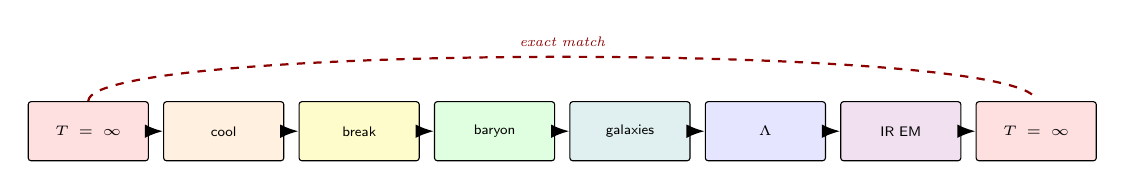
\begin{tikzpicture}[
  font=\sffamily\tiny,
  box/.style={draw, rounded corners=1pt, align=center, inner sep=2.5pt,
    text width=1.35cm, minimum height=0.75cm},
  arr/.style={-{Latex}, thick}
]
\node[box, fill=red!12] (a) {$T=\infty$};
\node[box, fill=orange!12, right=0.18cm of a] (b) {cool};
\node[box, fill=yellow!20, right=0.18cm of b] (c) {break};
\node[box, fill=green!12, right=0.18cm of c] (d) {baryon};
\node[box, fill=teal!12, right=0.18cm of d] (e) {galaxies};
\node[box, fill=blue!10, right=0.18cm of e] (f) {$\Lambda$};
\node[box, fill=violet!12, right=0.18cm of f] (g) {IR EM};
\node[box, fill=red!12, right=0.18cm of g] (h) {$T=\infty$};
\draw[arr] (a)--(b); \draw[arr] (b)--(c); \draw[arr] (c)--(d);
\draw[arr] (d)--(e); \draw[arr] (e)--(f); \draw[arr] (f)--(g); \draw[arr] (g)--(h);
\draw[red!55!black, dashed, thick] (a.north) .. controls +(0,0.75) and +(0,0.75) .. (h.north)
  node[midway, above, font=\tiny\itshape] {exact match};
\end{tikzpicture}%
}
\end{center}

\section{Phase anchors (order of magnitude)}
\begin{itemize}
\item Hot EM beginning: incoming radiation branch of HCCC conformal matching.
\item EW concurrency: $t_\diamond\sim10^{-11}\,\mathrm{s}$ when $\Td>T_*$.
\item Early galaxies: nonlinear contrast by $z\simeq14$ possible for strong
  gravitational response coupling (timing, not abundances).
\item Late $\Lambda$-like term: dilution-driven criticality and vacuum-like attractor.
\item End of aeon: infrared-first EM Hysterical instability $\to$ active crossover.
\end{itemize}

\section{Galactic subplot}
\begin{enumerate}
\item \textbf{Critical gravity.} Positive matter--response coupling $\Rightarrow$
  supercritical frozen Jacobian; growth above ordinary dust.
\item \textbf{Capacity.} Formation/retention conjecture:
  $Q\gtrsim O(\sqrt{\Mb})$.
\item \textbf{Relaxation / stability.} Capacity--filling ODE $\to$ stable attractor
  $Q^{2}\propto\Mb$ (hence BTFR $\vf^{4}\propto\Mb$ with flat $\vf^{2}=CQ$).
\item \textbf{Spherical $\to$ oblate.} Leading halo $n\propto Q/r^{2}$ is spherical;
  first angular correction is an oblate quadrupole.
\item \textbf{Size--mass.} Isotropic accretion $\Rightarrow R\propto\Mb^{5/12}$
  ($\alpha=5/12$).
\end{enumerate}

\section{What is not claimed}
Observed $\eta_B$ magnitude; galaxy abundances; saturated IR EM amplitude;
junction regularity; proof that Nature realises the whole cycle.
Those remain open or outside the inherited theorems.

\section{Pointer}
Full qualitative narrative, figures, and status table:
\texttt{paper\_14\_hysterical\_universe.tex}.
\end{document}
